\documentclass{standalone}

\usepackage[usenames,dvipsnames]{xcolor}
\usepackage{tikz}
\usepackage{pgfplots}
\usepackage{graphicx}
\usepackage{comment}

\pgfplotsset{compat=newest}
\pgfplotsset{
	legend style={
		font=\scriptsize, % Adjust font size
		nodes={scale=1.125, transform shape} % Scale down the legend
	}
}

\usetikzlibrary{shapes.geometric}

\definecolor{IBM1}{HTML}{648fff}
\definecolor{IBM2}{HTML}{785ef0}
\definecolor{IBM3}{HTML}{dc267f}
\definecolor{IBM4}{HTML}{fe6100}
\definecolor{IBM5}{HTML}{ffb000}
\definecolor{IBM6}{RGB}{051,117,056}

\definecolor{PTB1}{RGB}{046,037,133}
\definecolor{PTB2}{RGB}{051,117,056}
\definecolor{PTB3}{RGB}{093,168,153}
\definecolor{PTB4}{RGB}{148,203,236}
\definecolor{PTB5}{RGB}{220,205,125}
\definecolor{PTB6}{RGB}{194,106,119}

\definecolor{Okabe1}{RGB}{000,158,115}
\definecolor{Okabe2}{RGB}{000,114,178}
\definecolor{Okabe3}{RGB}{086,180,233}
\definecolor{Okabe4}{RGB}{230,159,000}
\definecolor{Okabe5}{RGB}{213,094,000}
\definecolor{Okabe6}{RGB}{204,121,167}

% Define a 5-point star as a TikZ style
\pgfdeclareplotmark{mystar}{
	\node[star,star point ratio=2.25,minimum size=8pt,
	inner sep=0pt,draw=Okabe2,fill=Okabe2!80,opacity=0.7] {};
}
\begin{document}
	\vspace{1cm}
		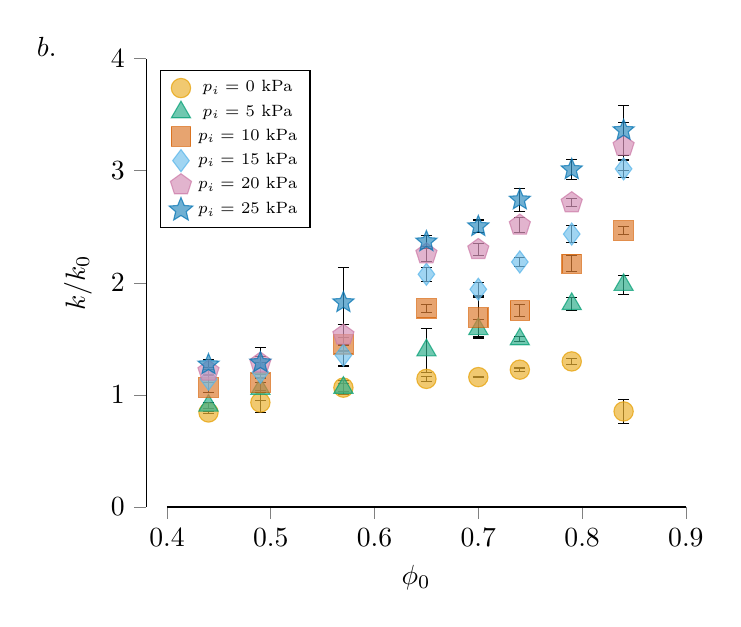
\begin{tikzpicture}
		\begin{axis}[
			%title={Diagonal View - 20 mm section},
			title={$b.$},
			title style={yshift=-2ex, xshift=-31ex},
			enlargelimits=false,
			tick pos=left, %
			tick align=outside, %
			axis line style={opacity=0}, %
			after end axis/.code={
				\draw ({rel axis cs:0,0}
				-|{axis cs:0.4,0}) % xmin (line starts here)
				-- ({rel axis cs:0,0}
				-|{axis cs:0.9,0}); % xmax (line stops here)
				\draw ({rel axis cs:0,0}
				|-{axis cs:0,0}) % ymin (line starts here)
				-- ({rel axis cs:0,0}
				|-{axis cs:0,4}); % ymax (line stops here)
			},
			xlabel={$\phi_0$},
			ylabel={$k/k_0$},
			xmin=0.38, xmax=0.9,
			ymin=0, ymax=4,
			xtick = {0.4, 0.5, 0.6, 0.7, 0.8, 0.9},
			xticklabels = {0.4, 0.5, 0.6, 0.7, 0.8, 0.9},
			legend style={
				at={(0.025,0.975)},
				anchor=north west,
				fill=none
			},
			scatter/classes={
				a={mark=*, mark size=3.5pt, color = Okabe4, fill=Okabe4!80,opacity=0.7},
				b={mark=triangle*, mark size=4pt,color = Okabe1, fill=Okabe1!80,opacity=0.7},
				c={mark=square*, mark size=3.5pt,color = Okabe5, fill=Okabe5!80,opacity=0.7},
				d={mark=diamond*, mark size=4pt,color = Okabe3, fill=Okabe3!80,opacity=0.7},
				e={mark=pentagon*, mark size=4pt,color = Okabe6, fill=Okabe6!80,opacity=0.7},
				f={mark=mystar, mark size = 5pt, color = Okabe2, fill=Okabe2!80,opacity=0.7}
			}
			]
			\addplot[scatter,only marks,% 
			scatter src=explicit symbolic, % Needed for scatter class styling
			error bars/.cd,
			x dir=both, x explicit,
			y dir=both, y explicit
			] 
			table[y error index=2, meta=label] {
				x 	y 		yerr 	label
				0.44	0.84323997	0.005236148	a
				0.44	0.904955104	0.02824227	b
				0.44	1.065268913	0.045872941	c
				0.44	1.140800423	0.03175308	d
				0.44	1.212309632	0.033129986	e
				0.44	1.270545752	0.046189904	f
				0.49	0.931807817	0.090635549	a
				0.49	1.053849969	0.100370239	b
				0.49	1.109020767	0.069943889	c
				0.49	1.201581008	0.09091845	d
				0.49	1.283995783	0.139248924	e
				0.49	1.288688466	0.053293154	f
				0.57	1.064723137	0.059988067	a
				0.57	1.06399045	0.036379479	b
				0.57	1.45111311	0.059621025	c
				0.57	1.354710003	0.096583792	d
				0.57	1.532471222	0.093965966	e
				0.57	1.825042429	0.309890566	f
				0.65	1.143090691	0.020059427	a
				0.65	1.39798586	0.194958069	b
				0.65	1.772176852	0.03623527	c
				0.65	2.076446121	0.064114603	d
				0.65	2.257848344	0.069959253	e
				0.65	2.36773388	0.057582145	f
				0.70	1.158606699	0.003596807	a
				0.70	1.587639528	0.084812746	b
				0.70	1.691396914	0.174631526	c
				0.70	1.942062936	0.059276171	d
				0.70	2.297129314	0.050796693	e
				0.70	2.50335067	0.057180788	f
				0.74	1.225164045	0.015139063	a
				0.74	1.496457436	0.022679377	b
				0.74	1.753403628	0.049952383	c
				0.74	2.186082445	0.038587282	d
				0.74	2.514208885	0.06714445	e
				0.74	2.74127941	0.102101027	f
				0.79	1.298604656	0.029288686	a
				0.79	1.811118892	0.056731407	b
				0.79	2.169626903	0.072377155	c
				0.79	2.434817065	0.076790183	d
				0.79	2.714436666	0.036866689	e
				0.79	3.011595886	0.091064465	f
				0.84	0.852725021	0.108423653	a
				0.84	1.981368828	0.082178556	b
				0.84	2.466220409	0.037194089	c
				0.84	3.01683933	0.079138842	d
				0.84	3.219648958	0.213652064	e
				0.84	3.360726008	0.223425236	f
			};
			
			\addlegendentry[scale=0.75]{$p_i=$~0 kPa}
			\addlegendentry[scale=0.75]{$p_i=$~5 kPa}
			\addlegendentry[scale=0.75]{$p_i=$~10 kPa}
			\addlegendentry[scale=0.75]{$p_i=$~15 kPa}
			\addlegendentry[scale=0.75]{$p_i=$~20 kPa}
			\addlegendentry[scale=0.75]{$p_i=$~25 kPa}
			
			
		\end{axis}
		
	\end{tikzpicture}

	
\end{document}